
\section{Preliminaries}
\label{sec:background}
\newcommand{\satisfies}{\vdash_{\!\!s}}
\newcommand{\nsatisfies}{\nvdash_{\!\!s}}

To start formalization, we define \emph{provability} abstractly from a set of model elements.  We represent the implementation model as a set of formulas $\Gamma$  and the set of requirements $\Delta$.  Then given $T \subseteq \Gamma$ and $e \in \Delta$, we use the notation $T \vdash e$ to mean that $e$ is \emph{provable} given the set $T$.  We assume that the provability relation $\vdash$ is monotonic on the subset relation over $\Gamma$, that is, if $S \subseteq S' \subseteq \Gamma$ and $S \vdash r$, then $S' \vdash r$.  The monotonicity of the satisfaction relation means that, unless {\em all} elements of the implementation $\Gamma$ are required for a proof, there are multiple implementation sets $S \subset S' \subset \ldots \subset \Gamma$ that can satisfy a given requirement $r$.  However, we are primarily interested in {\em minimal} sets that satisfy $r$; tracing a requirement to the entire implementation is not particularly enlightening.  We call a minimal set of model elements a \emph{support set} for that requirement, and define the $SOS$ relation to associate support sets to requirements.

$$ \ SOS(r, S) \equiv S \vdash r~ \land   (\neg\exists S'\ .\ S' \subset S \wedge S' \vdash r) $$

$SOS$ maps a requirement to a support set. However, there could be many support sets for a requirement. To capture that notion, we define, \emph{all support sets ($ASOS$)} for a requirement as an association to all its sets of support.


$$ ASOS(r) \equiv  \{\ S | S \subseteq \Gamma \land (r,S) \in SOS\ \} $$

The set of $ASOS$-es for all requirements represents the complete traceability of the system. Establishing $ASOS$ for a requirement, one gets a clear picture of the all possible ways that requirement is satisfied. This information helps categorize each target artifact into one of the following groups for that requirement.  The relationships are illustrated graphically in Fig.~\ref{fig:maymust}, and explained formally below.

\begin{itemize}
  \item \textbf{MUST} elements - target artifacts that are present in all the support sets for a requirement.
      %$$ MUST_x = \{\forall i (S_xi \in \Sigma_x) \mid \bigcap S_xi \}$$
      $$ MUST (r) = \bigcap \ ASOS(r) $$

  \item \textbf{MAY} elements - target artifacts that are used in some, but not all, support sets.
      $$MAY(r) = (\bigcup ASOS (r)) \setminus MUST (r) $$

  \item \textbf{IRRELEVANT} elements - target artifacts that are not in any of the support sets. $$IRR(r) = \Gamma \setminus (\bigcup ASOS (r))$$
\end{itemize}

Given requirement $r$, functions MUST, MAY, and IRR partition set $\Gamma$ into three disjoint sets \emph{must}, \emph{may}, and \emph{irrelevant}, respectively. This categorization helps to identify the role and relevance of each target artifact in satisfying a requirement. The \emph{must} set contains those target artifacts that are absolutely necessary for the requirement satisfaction. Hence, any change to these elements will most likely impact on each other. On the other hand, elements in the \emph{may} set indicate those target artifacts that satisfy the requirement in one of the possible ways.  Any change to just one of these elements will not affect the satisfaction of that requirement. The IRR function maps a requirement to the elements that never affect the satisfaction of the requirement \cite{Murugesan16:renext}.

\begin{figure}[htb]
\begin{center}
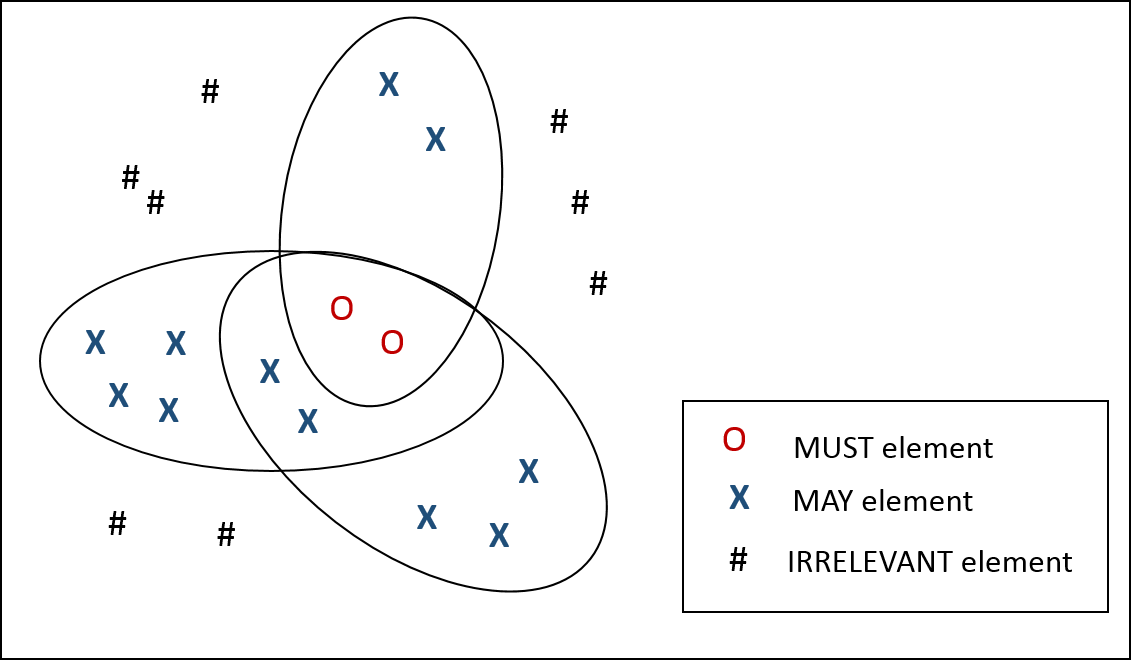
\includegraphics[width=\columnwidth]{figs/may_must.png}
\caption{A visual example of partitioning the implementation model}\label{fig:maymust}
\end{center}
\end{figure}

In light of this intuition, we define existing coverage notions in the literature, which are based on the idea of \emph{mutation}. Then, later, we explore some novel notions of coverage based on the idea of support sets.  More formally, mutation, denoted by $f_m$, is a relation that maps $\Gamma$ to set $S \subset \Gamma$ (written as $f_m (S)$). The range of $f_m$ for $\Gamma$ is denoted by $M$.

In general, requirement completeness can be defined with regard to the notion of \emph{coverage}. In fact, the way that coverage is formalized plays a key part in the strength/ effectiveness of a method for the assessment of completeness. Requirement completeness can be judged on a fraction called \emph{coverage score}, the closer to 1 the score is, the more complete the specification is. 

\begin{definition}{\emph{Coverage:}}
  \label{def:coverage}
   Any notion of coverage can be formalized as a function $\psi$ such that,
   $\forall r \in \Delta, \varphi \in \Gamma$, if $\varphi$ is covered by $r$ then $\psi (r, \varphi) = true$, denoted by $\psi (r) \preccurlyeq \varphi$, otherwise  $\psi (r, \varphi) = false$, denoted by $\psi (r) \nprec \varphi$.
\end{definition}

\begin{definition} {\emph{Coverage based on single mutation \cite{chockler2010coverage, chockler_coverage_2003}:}}
  \label{def:coverage1}
   $\forall r \in \Delta$, 
   $\varphi \in \Gamma$, 
   $\psi (r) \preccurlyeq \varphi$ 
   iff $\Gamma \vdash r$ and
   $f_m (\Gamma \setminus \{ \varphi \}) \nvdash r$. Otherwise, $\psi (r) \nprec \varphi$.
\end{definition}

For the sake of simplicity, we refer to the coverage function 
formalized in Definition \ref{def:coverage1} as $\psi_{sm}$.

Using $\psi_{sm}$, the coverage score of specification $r$ is computed by $$\frac{\sum_{\varphi \in \Gamma} f_m (\Gamma \setminus \{ \varphi \}) \nvdash r}{|\Gamma|}$$
Usually, a mutation is an atomic change to the design whose effect is not masked by other modifications, which means simultaneous mutations may lead to masking the changes. However,
it is possible to define the coverage notion with regard to all possible mutations, although it would be also very expensive and impractical \cite{chockler2001practical}. \ela{Mike, is the citation correct?}.
For a coverage function based on all mutations, the coverage score is calculated by 
$$ \frac{\sum_{S \in M} f_m (S) \nvdash r}{|\Gamma| |M|}$$ 

Since coverage is quite well-studied in testing, to compare it against the corresponding notions in formal verification, it is worth pointing out one of the most common coverage notions in testing known as \emph{decision coverage (DC)}, where a decision is considered as a boolean expression.  Given a test suit $T$, DC checks if every decision has taken all possible outcomes (i.e. $true$ and $false$) at least once. In testing, user has to furnish each requirement with some test cases, which is formalized as $R_m : \Delta \rightarrow 2^T$. Then coverage is measured using an over-approximation $T_m : T \times 2^\Gamma \times 2^\Delta \rightarrow 2^\Gamma$ as follows: $$\frac{|\bigcup_{t \in T} T_m (t, \Gamma)|}{|\Gamma|}$$ \ela{cite the paper Mike told. Also I'm not so sure of what I wrote. please verify.}




